%\frameT{Relations and Orderings}{
%  \begin{block}{Binary Relations}
%		Let $O$ be a set of objects. A \tit{binary relation} $\succeq$ over $O$ is a
%		collection of ordered pairs of objects in $O$; that is,
%		\begin{center}
%			$\succeq \; \subseteq O \times O$.
%		\end{center}
%  \end{block}
%
%	Properties of binary relations related to preferences:
%	\begin{enumerate}
%		\item Reflexivity: $\forall o \in O$, $o\succeq o$.
%		\item Irreflexivity: $\forall o \in O$, $o\not\succeq o$.
%		\item Totality: $\forall o_1,o_2$, $o_1\succeq o_2$ or $o_2\succeq o_1$.
%		\item Transitivity: $\forall o_1,o_2,o_3$, if $o_1\succeq o_2$ and $o_2\succeq o_3$, then $o_1\succeq o_3$.
%		\item Symmetry: $\forall o_1,o_2$, if $o_1\succeq o_2$, then $o_2\succeq o_1$.
%		%\item Asymmetry: $\forall o_1,o_2$, if $o_1\succeq o_2$, then $o_2\not\succeq o_1$.
%		\item Antisymmetry: $\forall o_1,o_2$, if $o_1\succeq o_2$ and $o_2\succeq o_1$, then $o_1=o_2$.
%	\end{enumerate}
%}

\frameT{Relations and Orderings}{
  \begin{block}{Binary Relations}
		Let $O$ be a set of objects. A \tit{binary relation} $R$ over $O$ is a
		collection of ordered pairs of objects in $O$; that is,
		\begin{center}
			$R \subseteq O \times O$.
		\end{center}
  \end{block}

	Properties of binary relations related to preferences:
	{\small
	\begin{enumerate}
		\item Reflexivity: $\forall o \in O$, $(o,o) \in R$.
		\item Irreflexivity: $\forall o \in O$, $(o,o) \not \in R$.
		\item Totality: $\forall o_1,o_2$, $(o_1,o_2) \in R$ or $(o_2,o_1) \in R$.
		\item Transitivity: $\forall o_1,o_2,o_3$, if $(o_1,o_2) \in R$ 
					and $(o_2,o_3) \in R$, then $(o_1,o_3) \in R$.
		\item Symmetry: $\forall o_1,o_2$, if $(o_1,o_2) \in R$, then $(o_2,o_1) \in R$.
		\item Antisymmetry: $\forall o_1,o_2$, if $(o_1,o_2) \in R$ 
					and $(o_2,o_1) \in R$, then $o_1=o_2$.
	\end{enumerate}
	}
}

\frameT{Relations and Orderings}{
  \begin{block}{Orderings}
		%A binary relation $\succeq$ over $O$ 
		$\succeq$
		is a \tit{partial preorder} if it is reflexive and
		transitive, a \tit{total preorder} if it is a partial preorder and total, 
		a \tit{partial order} if it is a partial preorder and antisymmetric, and 
		a \tit{total order} if it is a partial order and total.
  \end{block}

	\vspace{-0.3cm}

	\begin{figure}[ht]
	   \small
	  \centering
    \begin{subfigure}[b]{0.45\textwidth}
	  	\centering
		  \begin{tikzpicture}[->,>=stealth',node distance=1.5cm,main node/.style={circle,draw,font=\small}]
		    \node[main node,inner sep=0pt] (1)                    {$o_1,\!o_5$};
				\node[main node,inner sep=0pt] (2) [below left of=1]  {$o_2,\!o_6$};
		  	\node[main node,inner sep=0pt] (3) [below right of=1] {$o_3,\!o_7$};
		  	\node[main node,inner sep=0pt] (4) [below right of=2] {$o_4,\!o_8$};
		
		    \path[every node/.style={font=\sffamily\small}]
		      (4) edge (2)
		      (4) edge (3)
		      (2) edge (1)
		      (3) edge (1)
		      (4) edge (1)
					(1) edge [loop above] (1)
					(2) edge [loop left] (2)
					(3) edge [loop right] (3)
					(4) edge [loop below] (4);
		  \end{tikzpicture}
      \caption{partial preorder}
    \end{subfigure}
    \begin{subfigure}[b]{0.45\textwidth}
	  	\centering
		  \begin{tikzpicture}[->,>=stealth',node distance=1.1cm,main node/.style={circle,draw,font=\small}]
		    \node[main node,inner sep=0pt] (1)              {$o_1,\!o_5$};
				\node[main node,inner sep=0pt] (2) [below of=1] {$o_2,\!o_6$};
		  	\node[main node,inner sep=0pt] (3) [below of=2] {$o_3,\!o_7$};
		  	\node[main node,inner sep=0pt] (4) [below of=3] {$o_4,\!o_8$};
		
		    \path[every node/.style={font=\sffamily\small}]
		      (4) edge (3)
		      (4) edge [bend left] (2)
		      (4) edge [bend left] (1)
		      (3) edge (2)
		      (3) edge [bend left] (1)
		      (2) edge (1)
					(1) edge [loop right] (1)
					(2) edge [loop right] (2)
					(3) edge [loop right] (3)
					(4) edge [loop right] (4);
		  \end{tikzpicture}
      \caption{total preorder}
    \end{subfigure}
	\end{figure}
}

\frameT{Relations and Orderings}{
  \begin{block}{Orderings}
		%A binary relation $\succeq$ over $O$ 
		$\succeq$
		is a \tit{partial preorder} if it is reflexive and
		transitive, a \tit{total preorder} if it is a partial preorder and total, 
		a \tit{partial order} if it is a partial preorder and antisymmetric, and 
		a \tit{total order} if it is a partial order and total.
  \end{block}

	\vspace{-0.3cm}

	\begin{figure}[ht]
	   \small
	  \centering
    \begin{subfigure}[b]{0.45\textwidth}
	  	\centering
		  \begin{tikzpicture}[->,>=stealth',node distance=1.5cm,main node/.style={circle,draw,font=\small}]
		    \node[main node] (1) {$o_1$};
				\node[main node] (2) [below left of=1] {$o_2$};
		  	\node[main node] (3) [below right of=1] {$o_3$};
		  	\node[main node] (4) [below right of=2] {$o_4$};
		
		    \path[every node/.style={font=\sffamily\small}]
		      (4) edge (2)
		      (4) edge (3)
		      (2) edge (1)
		      (3) edge (1)
		      (4) edge (1)
					(1) edge [loop above] (1)
					(2) edge [loop left] (2)
					(3) edge [loop right] (3)
					(4) edge [loop below] (4);
		  \end{tikzpicture}
      \caption{partial order}
    \end{subfigure}
    \begin{subfigure}[b]{0.45\textwidth}
	  	\centering
		  \begin{tikzpicture}[->,>=stealth',node distance=1cm,main node/.style={circle,draw,font=\small}]
		    \node[main node] (1) {$o_1$};
				\node[main node] (2) [below of=1] {$o_2$};
		  	\node[main node] (3) [below of=2] {$o_3$};
		  	\node[main node] (4) [below of=3] {$o_4$};
		
		    \path[every node/.style={font=\sffamily\small}]
		      (4) edge (3)
		      (4) edge [bend left] (2)
		      (4) edge [bend left] (1)
		      (3) edge (2)
		      (3) edge [bend left] (1)
		      (2) edge (1)
					(1) edge [loop right] (1)
					(2) edge [loop right] (2)
					(3) edge [loop right] (3)
					(4) edge [loop right] (4);
		  \end{tikzpicture}
      \caption{total order}
    \end{subfigure}
	\end{figure}
}

%\frameT{Relations and Orderings}{
%  \begin{block}{Preference Relations}
%		Let $\succeq$ be a preference relation that is a partial preorder over $O$.
%		We say that $o_2$ is \tit{weakly preferred} to $o_1$ if $o_1 \succeq o_2$,
%		that $o_2$ is \tit{strictly preferred} ($\succ$) to $o_1$ if $o_1 \succeq o_2$ and
%		$o_2 \not \succeq o_1$, that $o_1$ is \tit{equivalent} ($\approx$) with $o_2$ 
%		if $o_1 \succeq o_2$ and $o_2 \succeq o_1$, and 
%		that $o_1$ is \tit{incomparable} ($\sim$) with $o_2$ if 
%		$o_1 \not \succeq o_2$ and $o_2 \not \succeq o_1$.
%  \end{block}
%
%	\vspace{-0.3cm}
%
%	\begin{figure}[ht]
%	   \small
%	  \centering
%    \begin{subfigure}[b]{0.45\textwidth}
%	  	\centering
%		  \begin{tikzpicture}[->,>=stealth',node distance=1.5cm,main node/.style={circle,draw,font=\small}]
%		    \node[main node,inner sep=1.2pt] (1)                    {$o_{1,5}$};
%				\node[main node,inner sep=1.2pt] (2) [below left of=1]  {$o_{2,6}$};
%		  	\node[main node,inner sep=1.2pt] (3) [below right of=1] {$o_{3,7}$};
%		  	\node[main node,inner sep=1.2pt] (4) [below right of=2] {$o_{4,8}$};
%		
%		    \path[every node/.style={font=\sffamily\small}]
%		      (4) edge (2)
%		      (4) edge (3)
%		      (2) edge (1)
%		      (3) edge (1)
%		      (4) edge (1)
%					(1) edge [loop above] (1)
%					(2) edge [loop left] (2)
%					(3) edge [loop right] (3)
%					(4) edge [loop below] (4);
%		  \end{tikzpicture}
%			\vspace{-0.3cm}
%      \caption{partial preorder}
%    \end{subfigure}
%    \begin{subfigure}[b]{0.45\textwidth}
%	  	\centering
%			\begin{tikzpicture}[->,>=stealth,node distance=0.5cm,main node/.style={rectangle,font=\small}]
%		    \node[main node] (1)              {$o_1 \succeq o_5$,};
%		    \node[main node] (2) [below of=1] {$o_2 \succ o_4$,};
%		    \node[main node] (3) [below of=2] {$o_4 \approx o_8$,};
%		    \node[main node] (4) [below of=3] {$o_6 \sim o_7$.};
%		    \node[main node] (5) [below of=4] {};
%		    \node[main node] (6) [below of=5] {};
%		  \end{tikzpicture}
%			\vspace{-0.3cm}
%      \caption{preferences}
%    \end{subfigure}
%	\end{figure}
%}

\frameT{Relations and Orderings}{
  \begin{block}{Preference Relations}
		Let $\succeq$ be a preference relation that is a total preorder over $O$.
		We say that $o_1$ is \tit{weakly preferred} to $o_2$ if $o_1 \succeq o_2$,
		that $o_1$ is \tit{strictly preferred} ($\succ$) to $o_2$ if $o_1 \succeq o_2$ and
		$o_2 \not \succeq o_1$, and that $o_1$ is \tit{equivalent} ($\approx$) with $o_2$ 
		if $o_1 \succeq o_2$ and $o_2 \succeq o_1$.
  \end{block}

	\vspace{-0.22cm}

	\begin{figure}[ht]
	   \small
	  \centering
    \begin{subfigure}[b]{0.45\textwidth}
	  	\centering
		  \begin{tikzpicture}[->,>=stealth',node distance=1.1cm,main node/.style={circle,draw,font=\small}]
		    \node[main node,inner sep=0pt] (1)              {$o_1,\!o_5$};
				\node[main node,inner sep=0pt] (2) [below of=1] {$o_2,\!o_6$};
		  	\node[main node,inner sep=0pt] (3) [below of=2] {$o_3,\!o_7$};
		  	\node[main node,inner sep=0pt] (4) [below of=3] {$o_4,\!o_8$};
		
		    \path[every node/.style={font=\sffamily\small}]
		      (4) edge (3)
		      (4) edge [bend left] (2)
		      (4) edge [bend left] (1)
		      (3) edge (2)
		      (3) edge [bend left] (1)
		      (2) edge (1)
					(1) edge [loop right] (1)
					(2) edge [loop right] (2)
					(3) edge [loop right] (3)
					(4) edge [loop right] (4);
		  \end{tikzpicture}
      \caption{total preorder}
    \end{subfigure}
    \begin{subfigure}[b]{0.45\textwidth}
	  	\centering
			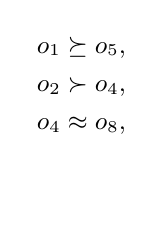
\begin{tikzpicture}[->,>=stealth,node distance=0.5cm,main node/.style={rectangle,font=\small}]
		    \node[main node] (1)              {$o_1 \succeq o_5$,};
		    \node[main node] (2) [below of=1] {$o_2 \succ o_4$,};
		    \node[main node] (3) [below of=2] {$o_4 \approx o_8$,};
		    \node[main node] (4) [below of=3] {};
		    \node[main node] (5) [below of=4] {};
		  \end{tikzpicture}
			\vspace{-0.3cm}
      \caption{preferences}
    \end{subfigure}
	\end{figure}
}

\frameT{Combinatorial Domains}
{
	\begin{block}{Combinatorial Domains}
	  Let $\cI$ be a finite set of attributes $\{X_1,\ldots,X_p\}$,
	  associated with a set of finite domains $\{\Dom(X_1),\ldots,\Dom(X_p)\}$ for each
	  attribute $X_i$.
	  A \tit{combinatorial domain} $\CD(\cI)$ is a set of \tit{objects}
		described by combinations of values from $\Dom(X_i)$:
	  \begin{center}
	    $\CD(\cI) = \prod_{X_i \in \cI} \Dom(X_i)$.
	  \end{center}
	\end{block}
}

\frameT{Combinatorial Domains: Example}{
	Domain of cars over set $\cI$ of $p$ binary attributes:
	\begin{enumerate}
		\item \tbf{BodyType}: \{mvan, sedan\}.
		\item \tbf{Capacity}: \{5, 7m\}.
		\item \tbf{Color}: \{blue, gray\}.
		\item[\vdots]
	\end{enumerate}

	\begin{center}
			$\CD(\cI) = 
				\underbrace{\{\langle\text{sedan, 5, blue, }\ldots\rangle, 
				\langle\text{mvan, 7m, gray, }\ldots\rangle, \ldots\}}_{\text{\large $2^p$ objects, too many!}}$.
	\end{center}

%	\begin{center}
%		\begin{align*} 
%			\CD(\cI) = \{&<\text{sedan, 4, blue, }\ldots>, \\
%								 &<\text{mvan, 6m, gray, }\ldots>, \\
%								 &\ldots\}.
%		\end{align*}
%	\end{center}
}

%\frameT{Computational Complexity}{
%	\begin{enumerate}
%		\item $P$, $\NP$, $\coNP$: We typically believe that $P \subset \NP$.
%		%\item $\coNP$: problems whose complements are in $\NP$.
%		\item $\deltap{2}$: $P^\NP$, $\sigmap{2}$: $\NP^\NP$, and $\pip{2}$: $\coNP^\NP$.
%		\item $C$-complete: hardest decision problems in class $C$.
%		%\item A decision problem $L$ is $C$-hard if $L' \leq_p L$ for every $L'$ in class $C$.
%		%\item A decision problem $L$ is $C$-complete if $L$ is in class $C$ and $L$ is $C$-hard.
%	\end{enumerate}
%}

%\frameT{Computational Complexity}{
%	\begin{enumerate}
%		\item $P$, $\NP$, $\coNP$: We typically believe that $P \subset \NP$ and $P \subset \coNP$.
%		%\item $\coNP$: problems whose complements are in $\NP$.
%		\item $\deltap{2}$: $P^\NP$, $\sigmap{2}$: $\NP^\NP$, and $\pip{2}$: $\coNP^\NP$.
%		\item $C$-complete: hardest decision problems in class $C$.
%		%\item A decision problem $L$ is $C$-hard if $L' \leq_p L$ for every $L'$ in class $C$.
%		%\item A decision problem $L$ is $C$-complete if $L$ is in class $C$ and $L$ is $C$-hard.
%	\end{enumerate}
%
%	\vspace{-0.3cm}
%
%	\begin{figure}[ht!]
%	  \centering
%	    \includegraphics[width=0.5\textwidth]{figs/Preliminary/comp_diagram.pdf}
%	  \caption{Computational complexity diagram}
%	\end{figure}
%}

\frameT{Combinatorial Domains: Example}{
	Domain of cars:
	\begin{enumerate}
		\item \tbf{BodyType}: \{mvan, sedan, sport, suv\}.
		\item \tbf{Capacity}: \{2, 5, 7m\}.
		\item \tbf{Color}: \{black, blue, gray, red, white\}.
		\item \tbf{LuggageSize}: \{big, med, small\}.
		\item \tbf{Make}: \{bmw, ford, honda, vw\}.
		\item \tbf{Price}: \{low, med, high, vhigh\}.
		\item \tbf{Safety}: \{low, med, high\}.
	\end{enumerate}
}

\frameT{Single Agent}{
	\begin{figure}[ht!]
	  \centering
	    \includegraphics[width=0.95\textwidth]{figs/Cars/individual.png}
	  \caption{Dominance and Optimization}
	\end{figure}
}

\frameT{Multi-Agent}{
	\begin{figure}[ht!]
	  \centering
	    \includegraphics[width=0.5\textwidth]{figs/Cars/group.png}
	  \caption{Social Choice and Welfare}
	\end{figure}
}

\frameT{Research Problems of Interest}{
	\begin{enumerate}
		\item Preference representation formalisms to compactly model qualitative preferences
					over combinatorial domains.
		\item Preference elicitation and learning methods to cast preferences of agents 
					as a theory in a preference formalism.
		\item Preference reasoning tasks:
		\begin{itemize}
			\item Dominance and optimization
			\item Manipulation: better off by misreporting preferences.
		\end{itemize}
	\end{enumerate}
}
